% ====================================================================
%+
% SECTION:
%    SolarSystem_PHA.tex
%
% CHAPTER:
%    solarsystem.tex
%
% ELEVATOR PITCH:
%    Discovery of PHAs in particular. Discussion of wider 'impacts'.
%
%-
% ====================================================================

\section{Discovery of Potentially Hazardous Asteroids}
\def\secname{\chpname:phas}\label{sec:\secname}

\credit{ivezic},
\credit{rhiannonlynne}.

The U.S. Congress has given a mandate to NASA to implement a
Near-Earth Object (NEO) Survey program to detect, track, catalog, and
characterize the physical characteristics of near-Earth objects equal
to or greater than 140 meters in diameter\footnote{See
\url{http://www.gpo.gov/fdsys/pkg/PLAW-109publ155/pdf/PLAW-109publ155.pdf}}. The
goal is to achieve a completeness of 90\%. In recent practice, adopted
here, the completeness is evaluated for a subset of NEOs called
Potentially Hazardous Asteroids\footnote{Potentially Hazardous
Asteroids (PHAs) are defined as asteroids with a minimum orbit
intersection distance (MOID) of 0.05 AU or less.} (PHA), with
H$\le$22, where H is the absolute magnitude\footnote{Absolute
magnitude is the magnitude that an asteroid would have at a distance
of 1 AU from the Sun and from the Earth, viewed at zero phase
angle. This is an impossible configuration, of course, but the
definition is motivated by desire to separate asteroid physical
characteristics from the observing configuration.} in the Johnson's V
band.

The discovery criteria for PHAs follows the same guidelines and metrics found in the previous
section, \ref{sec:solarsystem:discovery}, but is worth discussing
separately to focus on its main figure
of merit - completeness for PHAs with H$\le$22 magnitudes.

% --------------------------------------------------------------------

\subsection{Target measurements and discoveries}
\label{sec:\secname:targets}

Using the same range of discovery criteria as in the previous section,
\ref{sec:solarsystem:discovery}, we can look at the differential and
cumulative completeness for a population of PHAs. For this sample of
PHAs, we pulled the orbits of 2,000 objects with MOID~$<= 0.05$~AU from 
the Grav S3M model \citep{2011PASP..123..423G}. These orbits were
then cloned over a range of $H$ values to evaluate the chances of
discovery for that orbit at each of those $H$ values. The differential
completeness as a function of $H$ is then simply the fraction of
objects which receive at least one set of observations which meet the
discovery criteria during the course of the survey. The cumulative
completeness is similar, but integrated over $H$ by assuming an $H$
distribution with a power-law index of $\alpha=0.3$. Both
differential and cumulative completeness are relevant metrics: the
former provides more insight in the behavior of a particular
simulation, while the latter is a metric given to NASA by the U.S.
Congress.

To match the NEO mandate, the cumulative completeness at $H$=22 can be
used as a figure of merit.

% --------------------------------------------------------------------

\subsection{Metrics}
\label{sec:\secname:metrics}

The metrics used here are the same as in
\ref{sec:solarsystem:discovery}, although run with different input populations.

% --------------------------------------------------------------------

\subsection{OpSim Analysis}
\label{sec:\secname:analysis}

The differential and cumulative completeness for the baseline survey,
\opsimdbref{db:baseCadence}, at a range of years is shown in
\autoref{fig:baselinePHA}. The baseline cadence achieves a cumulative completeness of 66\% for
H$\le$22 PHAs when requiring pairs of visits on 3 separate nights within 15 days. 
The differential completeness at $H$=22 for the same
survey is 49\%, 17\% lower due to increasing completeness toward
smaller $H$ (larger objects).

%%%%%%%%%%%%%%%%%%%%%%%%%%%
\begin{figure}[th]
%\vskip -1.1in
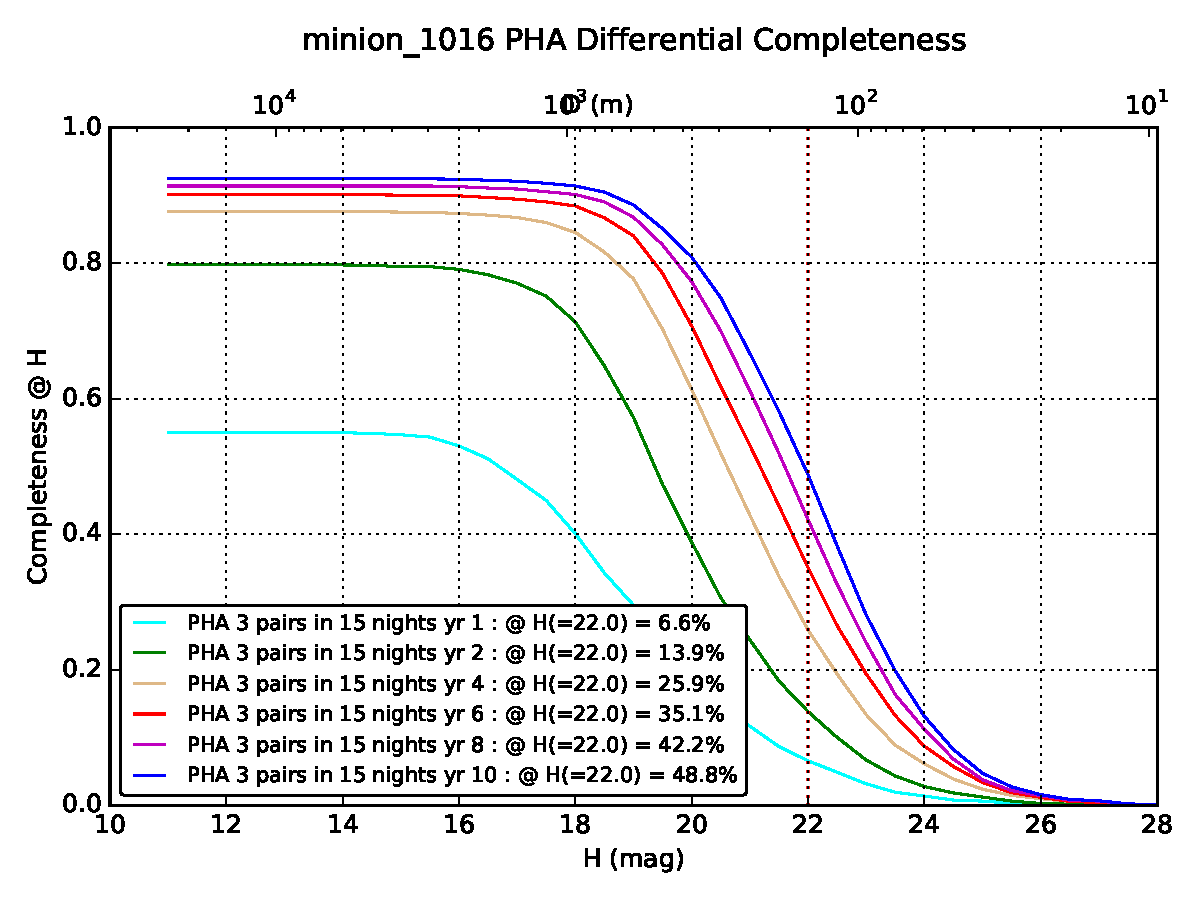
\includegraphics[angle=0,width=0.49\hsize:,clip]{figs/solarsystem/minion_1016_DifferentialCompleteness_PHA_3_pairs_in_15_nights_Years_1_to_10_MOOB_ComboMetricVsH}
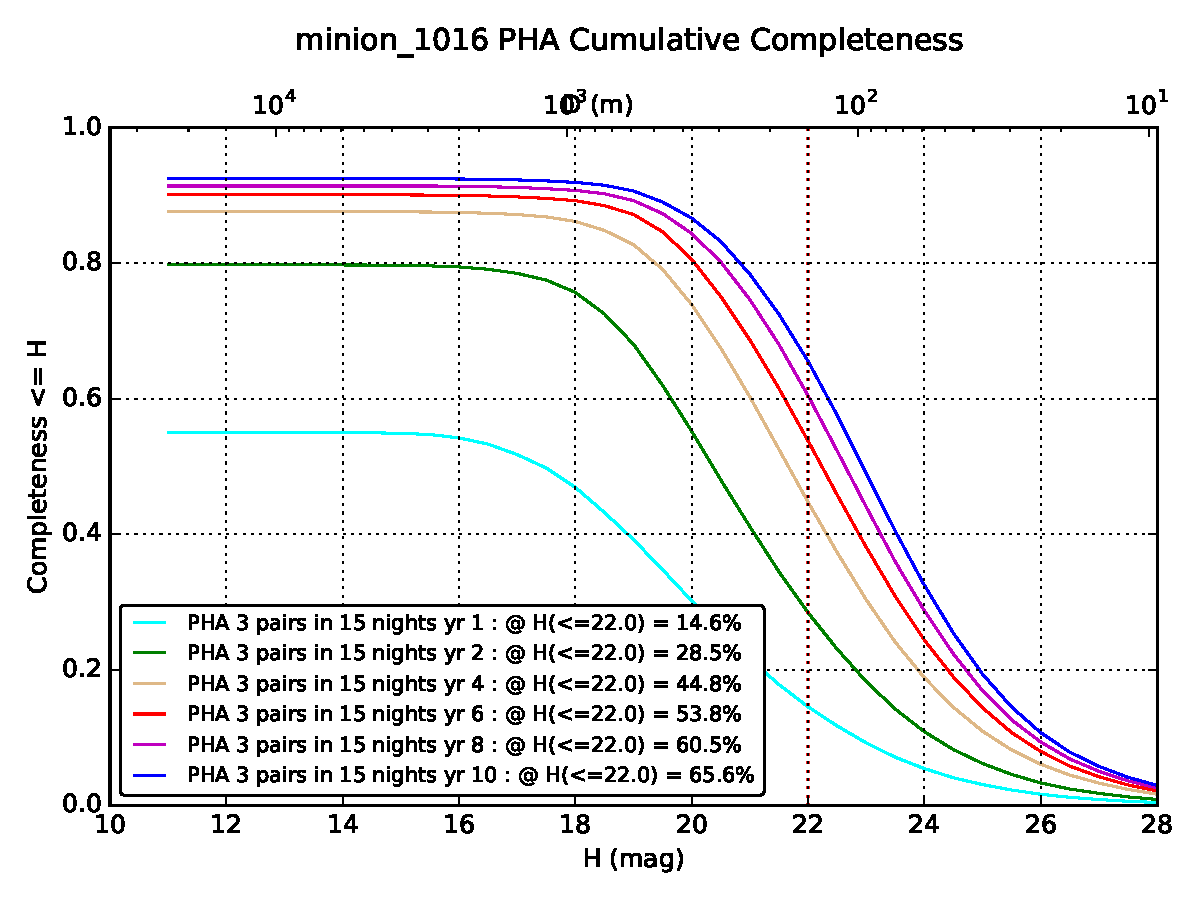
\includegraphics[angle=0,width=0.49\hsize:,clip]{figs/solarsystem/minion_1016_CumulativeCompleteness_PHA_3_pairs_in_15_nights_Years_1_to_10_MOOB_ComboMetricVsH}
%\vskip -1.2in
\caption{The PHA completeness for \opsimdbref{db:baseCadence}, as a function of the object's absolute
visual magnitude H on the horizontal axes (left: differential completeness at a given H;
right: cumulative completeness for all objects brighter than a given H), as it increases year over year.
The cumulative completeness for H$\le$22 NEOs (those with diameters larger than 140m)  for this
simulation is 66\% after 10 years.}
\label{fig:baselinePHA}
\end{figure}
%%%%%%%%%%%%%%%%%%%%%%%%%%%

We find that the PHA and NEO completeness are very similar for a given simulated survey and set of discovery criteria, as shown in \autoref{fig:neopha}.  The analysis of the various observing run strategies (singles, pairs, triples or quads of visits) described in the previous section thus applies to PHAs as well; while changing the discovery metric to triplets or quads significantly decreases completeness, simply changing the survey strategy has a softer effect, most likely due to current limitations of the simulated surveys.

%%%%%%%%%%%%%%%%%%%%%%%%%%%
\begin{figure}[bh]
%\vskip -1.2in
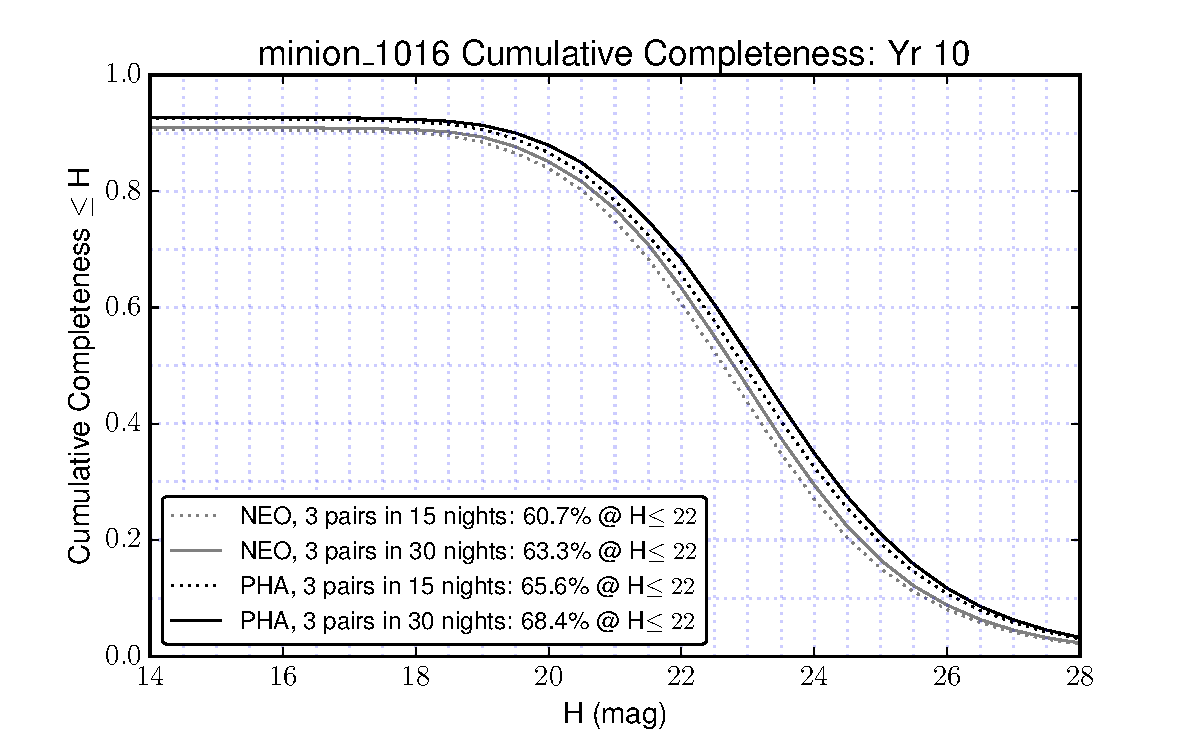
\includegraphics[angle=0,width=0.49\hsize:,clip]{figs/solarsystem/minion_1016_CumulativeCompleteness_NEO_and_PHA_Cumulative_Completeness}
%\vskip -1.3in
\caption{%
Comparison of the cumulative NEO and PHA completeness for the baseline cadence
\opsimdbref{db:baseCadence}.}
\label{fig:neopha}
\end{figure}
%%%%%%%%%%%%%%%%%%%%%%%%%%%

% ====================================================================
%
% \subsection{Conclusions}
%
% Here we answer the ten questions posed in
% \autoref{sec:intro:evaluation:caseConclusions}:
%
% \begin{description}
%
% \item[Q1:] {\it Does the science case place any constraints on the
% tradeoff between the sky coverage and coadded depth? For example, should
% the sky coverage be maximized (to $\sim$30,000 deg$^2$, as e.g., in
% Pan-STARRS) or the number of detected galaxies (the current baseline but
% with 18,000 deg$^2$)?}
%
% \item[A1:] ...
%
% \item[Q2:] {\it Does the science case place any constraints on the
% tradeoff between uniformity of sampling and frequency of  sampling? For
% example, a rolling cadence can provide enhanced sample rates over a part
% of the survey or the entire survey for a designated time at the cost of
% reduced sample rate the rest of the time (while maintaining the nominal
% total visit counts).}
%
% \item[A2:] ...
%
% \item[Q3:] {\it Does the science case place any constraints on the
% tradeoff between the single-visit depth and the number of visits
% (especially in the $u$-band where longer exposures would minimize the
% impact of the readout noise)?}
%
% \item[A3:] ...
%
% \item[Q4:] {\it Does the science case place any constraints on the
% Galactic plane coverage (spatial coverage, temporal sampling, visits per
% band)?}
%
% \item[A4:] ...
%
% \item[Q5:] {\it Does the science case place any constraints on the
% fraction of observing time allocated to each band?}
%
% \item[A5:] ...
%
% \item[Q6:] {\it Does the science case place any constraints on the
% cadence for deep drilling fields?}
%
% \item[A6:] ...
%
% \item[Q7:] {\it Assuming two visits per night, would the science case
% benefit if they are obtained in the same band or not?}
%
% \item[A7:] ...
%
% \item[Q8:] {\it Will the case science benefit from a special cadence
% prescription during commissioning or early in the survey, such as:
% acquiring a full 10-year count of visits for a small area (either in all
% the bands or in a  selected set); a greatly enhanced cadence for a small
% area?}
%
% \item[A8:] ...
%
% \item[Q9:] {\it Does the science case place any constraints on the
% sampling of observing conditions (e.g., seeing, dark sky, airmass),
% possibly as a function of band, etc.?}
%
% \item[A9:] ...
%
% \item[Q10:] {\it Does the case have science drivers that would require
% real-time exposure time optimization to obtain nearly constant
% single-visit limiting depth?}
%
% \item[A10:] ...
%
% \end{description}

\navigationbar
